\documentclass[12pt]{scrartcl}
\usepackage[english]{babel}
\usepackage{multirow}
\usepackage[default]{opensans}
\usepackage{sfmath} % sans font also for math
\usepackage[binary-units = true]{siunitx}
\usepackage{graphicx}
% defining the paper layout that no text overlaps with the header
\usepackage[
  top=35mm,
  headheight=25mm,
  headsep=3mm,
  bottom=30mm,
  left=25mm,
  right=25mm
]{geometry}

\usepackage[verbose]{placeins}
\usepackage{subfig}
\usepackage{latexsym}
\usepackage[centertags]{amsmath}
\usepackage{amssymb}
\usepackage[]{glossaries}

\graphicspath{{figures/}}
% custom header and footpage
\usepackage{scrpage2}
\pagestyle{scrheadings} % you have to set the custom layout
% Head
\ihead{M4.3} % left head
%\chead{}
\ohead{
\includegraphics[height=25mm]{figures/EUCALL.png}}
% Foot
\ifoot{
\includegraphics[height=13.4mm]{figures/EU.png}} % left foot
\cfoot{%
  \begin{minipage}{100mm}%
    \begin{scriptsize}%
      \normalfont{This project has received funding from the}
      \textit{European Union’s Horizon 2020 research and innovation programme}
      \normalfont{under grant agreement No 654220.}
    \end{scriptsize}%
  \end{minipage}%
} % center foot
\ofoot{\thepage} % right foot

\usepackage{booktabs}

%%%%%%%%%%%%%%%%%%%%%%%%%%%%%%%%%%%%%%%%%%%%%%%
%   BIBLIOGRAPHY SETTINGS
\usepackage[bibstyle=nature,sorting=none,maxnames=1000,eprint=false,
defernumbers=true, backend=biber]{biblatex}
\usepackage{hyperref}

\renewcommand*\finalnamedelim{, and\addspace}
\DeclareNameAlias{sortname}{last-first}
\renewcommand{\newunitpunct}{, }

\AtEveryBibitem{%
  \clearfield{day}%
  \clearfield{month}%
  \clearfield{endday}%
  \clearfield{endmonth}%
  \clearfield{issn}%
  \clearfield{issue}%
}
%convert titles to hyperlinks using doi
\ExecuteBibliographyOptions{doi=false} \newbibmacro{string+doi}[1]{%
  \iffieldundef{doi}{#1}{\href{http://dx.doi.org/\thefield{doi}}{#1}}}
  \DeclareFieldFormat*{title}{\usebibmacro{string+doi}{\mkbibemph{#1}}}

\addbibresource{references.bib}
\addbibresource{urls.bib}
\addbibresource{aux.bib}
\addbibresource{drafts.bib}
\addbibresource{contributions/HPL/sample.bib}
%%%%%%%%%%%%%%%%%%%%%%%%%%%%%%%%%%%%%%%%%%%%%%%
% GLOSSARY SETTINGS
\setacronymstyle{long-short}
\input{glossary}
\makeglossaries
%%%%%%%%%%%%%%%%%%%%%%%%%%%%%%%%%%%%%%%%%%%%%%%
% PDF SETTINGS
\usepackage{hyperref}                                             % for sophisticated linking of urls, dois, pictures, tables, etc.
\hypersetup{
    unicode=true,                                                 % non-Latin characters in Acrobat’s bookmarks
    pdftoolbar=true,                                              % show Acrobat’s toolbar?
    pdfmenubar=true,                                              % show Acrobat’s menu?
    pdffitwindow=false,                                           % window fit to page when opened
    pdftitle={M4.3: Interoperable simulations},                   % title
    pdfauthor={C. Fortmann-Grote},                                % author
    pdfsubject={EUCALL WP4 (SIMEX) Milestone 4.3},                % subject of the document
    pdfcreator={pdflatex},                                        % creator of the document
    pdfkeywords={EUCALL, SIMEX, simulations},                     % list of keywords
    pdfnewwindow=true,                                           % links in new PDF window
    colorlinks=true,                                             % false: boxed links; true: colored links
    linkcolor=blue,                                              % color of internal links (change box color with linkbordercolor)
    citecolor=blue,                                              % color of links to bibliography
    filecolor=blue,                                              % color of file links
    urlcolor=blue                                                % color of external links
}

% Zeilenabstand
\renewcommand{\baselinestretch}{1.2}


%%%%%%%%%%%%%%%%%%%%%%%%%%%%%%%%%%%%%%%%%%%%%%%
% DOCUMENT BODY
\begin{document}
\makeatletter
\begin{titlepage}
\thispagestyle{scrheadings}
\begin{center}
  $~$\\
  \vspace{2cm}
  \Huge{\textbf{WP 4 -- SIMEX\\[1cm]
    Milestone M4.3: Demonstration of interoperable simulations%
  }}\\
  \vspace{2cm}
  \large{Carsten Fortmann-Grote, Alexander Andreev, Ashutosh Sharma, Richard
    Briggs, Jan-Philipp Burchert, Marco Garten, Axel Huebl, Alexander Grund,
  Thomas Kluge, Sergey Yakubov, Michael Bussmann, and Adrian P. Mancuso}
  \vspace{1cm}
  \date{\today}
\end{center}
\vfill%
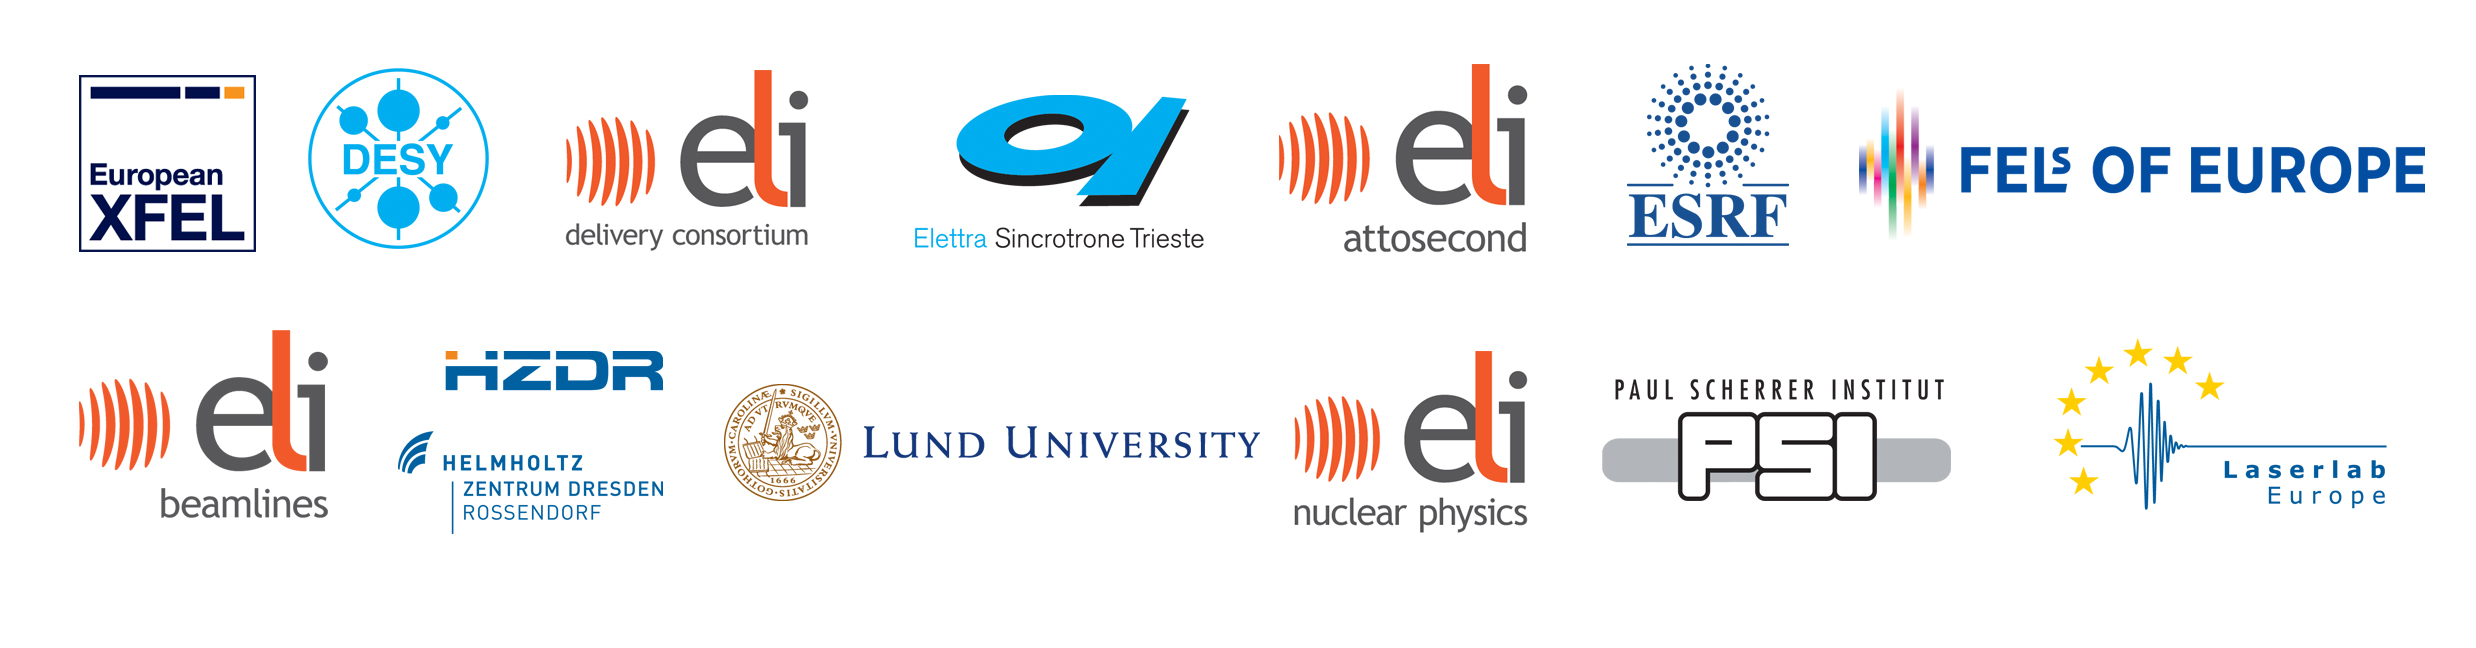
\includegraphics[width=\textwidth]{figures/PartnerLogos_2017}
\end{titlepage}
\makeatother
%
\tableofcontents
%
\newpage
%
\section{Summary}\label{sec:summary}
Milestone M4.3 (as detailed in Task 4.2.2) of the SIMEX
workpackage in EUCALL is the delivery of interoperable simulations
(Deliverable D4.3) with documented examples. We have chosen five
applications to demonstrate the interoperability of our simulation codes beyond
the first usage example, which is described in Milestone
M4.2~\cite{EUCALL_SIMEX_M4.2}.
%
\begin{enumerate}
  \item Simulation of diffraction of coherent x--rays delivered by an
    \gls{xfel}
    from high energy density matter created by short--pulse
    laser matter interaction (as detailed in Deliverable D4.1)
  \item Simulation of \gls{xafs} from long--pulse laser
    shocked warm dense matter at the synchrotron light source ESRF (as detailed
    in Deliverable D4.2).
  \item Coherent diffraction imaging of protein crystals
  \item X--ray Thomson Scattering from warm dense plasmas
  \item Laser--wakefield acceleration based coherent light sources
\end{enumerate}
%
These examples demonstrate the functionality and interoperability of all
simulation tools as demanded in Task 4.2.2.
Table~\ref{tab:simulation_capabilities} summarizes the available simulation
modules, the interfaced backengine simulation codes, and the relevant sections
of this report and external references where example applications can be found.

\begin{table}[!h]
  \begin{center}
    \scriptsize
    \caption{Demonstrated simulation capabilities}
    \label{tab:simulation_capabilities}
  \begin{tabular}[ht]{|l|l|l|l|}
    \hline
      \textbf{Task} &
      \textbf{Simulation capability} &
      \textbf{Simulation code}     &
      \textbf{Example references}    \\
    \hline
    \hline
      \multirow{3}{*}{X--ray sources}
      & XFEL source                     & FAST/XPD              & Refs~\cite{EUCALL_SIMEX_M4.1,EUCALL_SIMEX_M4.2,Fortmann-Grote2017}     \\
      & XFEL source                     & Genesis/Ocelot        & Sec.~\ref{sec:lwfa_source} \\
      & Synchrotron source              & ShadowOUI             & Sec.~\ref{sec:xafs}       \\
    \hline
    \multirow{2}{*}{Beam propagation}
      & Coherent wave propagaton        & WPG/SRW               & Refs~\cite{EUCALL_SIMEX_M4.1,EUCALL_SIMEX_M4.2,Fortmann-Grote2017}     \\
      & X--ray tracing                  & ShadowOUI             & Sec.~\ref{sec:xafs}       \\
    \hline
    \multirow{3}{*}{Photon--matter interaction}
      & Radiation damage to molecules   & XMDYN/XATOM           & Refs~\cite{EUCALL_SIMEX_M4.1,EUCALL_SIMEX_M4.2,Fortmann-Grote2017}     \\
      & Short--pulse optical laser      & PIConGPU              & Secs~\ref{sec:lwfa_source},\ref{sec:plasma_diffraction}, Ref.~\cite{EUCALL_SIMEX_D4.1}  \\
      & Long--pulse optical laser       & Esther Rad--hydro     & Sec.~\ref{sec:xafs} Ref.~\cite{Torchio2016}  \\
    \hline
    \multirow{5}{*}{Signal generation}
      & Nano-particle scattering        & singFEL               & Ref.~\cite{EUCALL_SIMEX_M4.1,EUCALL_SIMEX_M4.2,Fortmann-Grote2017}     \\

      & Plasma diffraction              & paraTAXIS             & Sec.~\ref{sec:plasma_diffraction},Ref.~\cite{EUCALL_SIMEX_D4.1,Kluge2016,
      Garten2017.zenodo.885033}  \\
      & XAFS                            & FEFF                  & Sec.~\ref{sec:xafs}, Refs~\cite{EUCALL_SIMEX_D4.2,Torchio2016,Harmand2015,Mazevet2014}  \\
      & Plasma XRTS                     & XRTScode              & Sec.~\ref{sec:xrts}, Ref.~\cite{Fortmann2009d}               \\
      & Nano--crystallography           & CrystFEL              & Sec.~\ref{sec:protein_sfx}         \\
    \hline
  \end{tabular}
  \end{center}
\end{table}

These codes are interfaced through the simulation platform ``simex\_platform'', which,
on the one side defines a python library to facilitate setup
and execution in a canonical way, and, on the other side, defines data interfaces
and formats to facilitate the passing of simulation data generated from one
module to the next.

\section{Coherent diffraction from high energy density matter}\label{sec:plasma_diffraction}
The interaction of \gls{uhi} lasers with solid matter at laser
pulse durations of few ten to hundred femtoseconds opens up the possibility to
study transient, non--equilibrium high energy density plasma processes on time
scales close to that of atomic processes with \glspl{xfel} with
nanometer resolution \cite{Kluge2016}, see also SIMEX Deliverable D4.1
\cite{EUCALL_SIMEX_D4.1}.
%
\begin{figure}[ht]
  \centering
  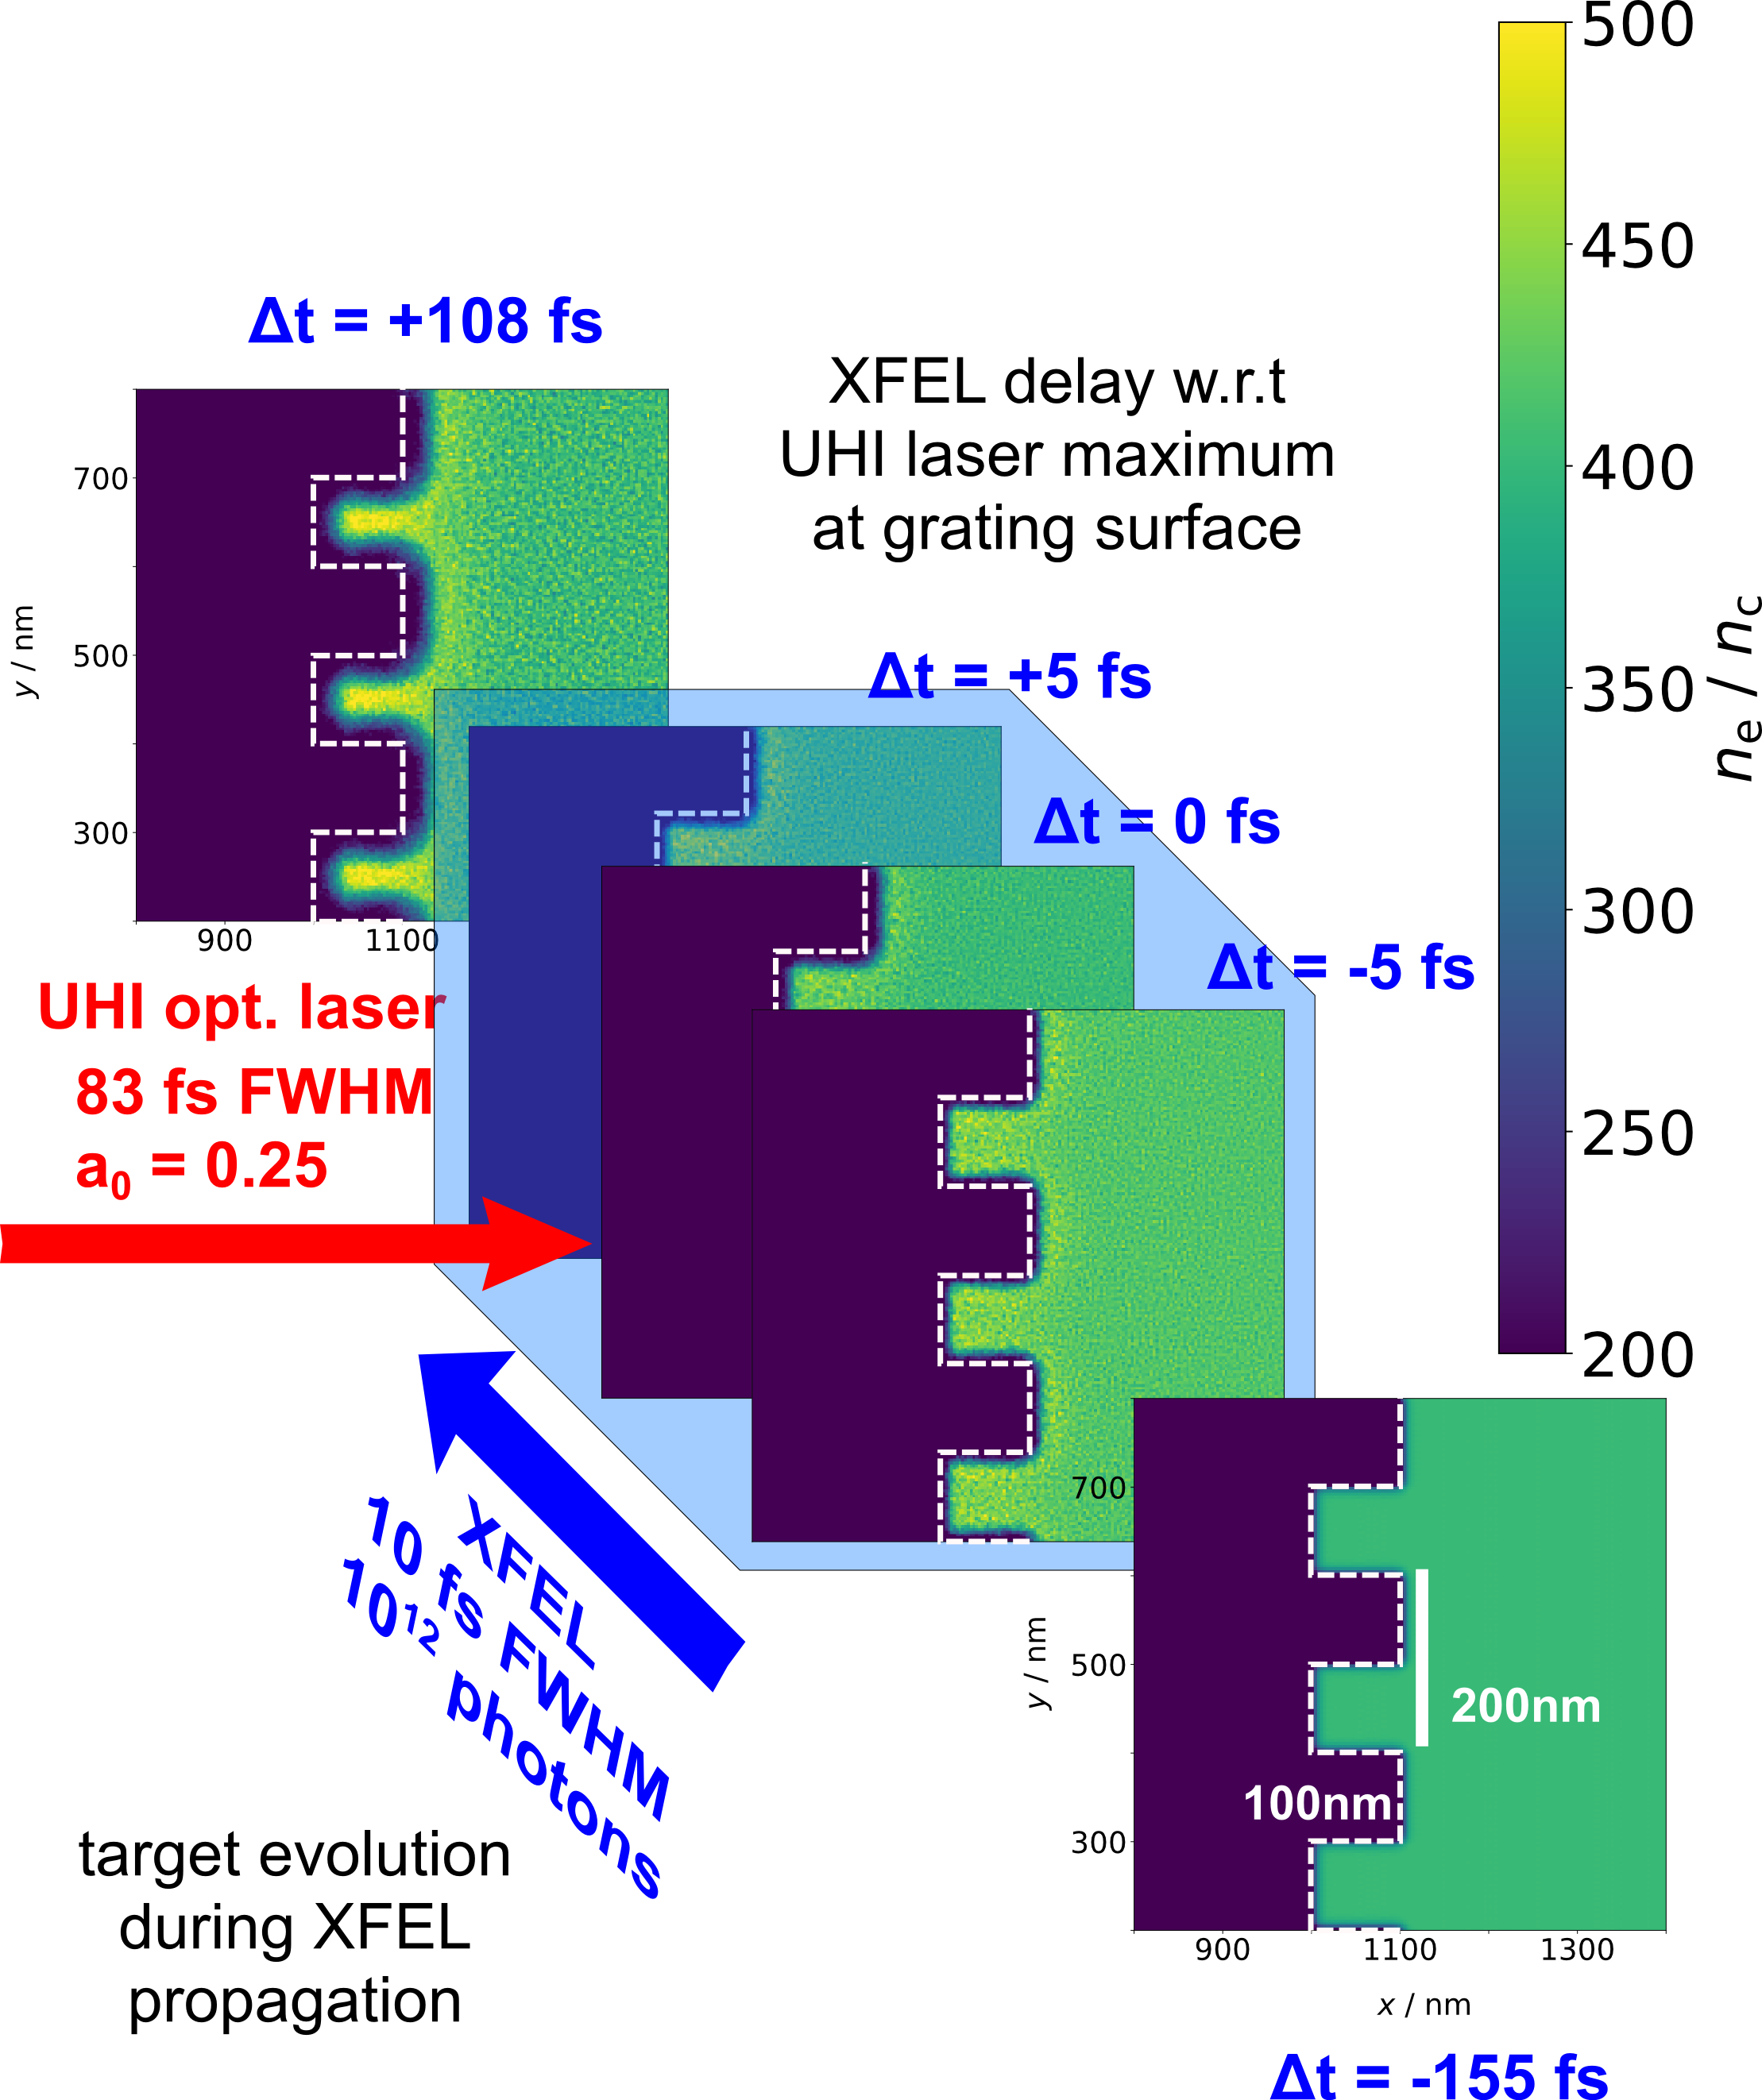
\includegraphics[width=.95\linewidth]{figures/scattering_geometry_v4.png}
  \caption{
    Scattering geometry with \gls{xfel} pulse perpendicular to optical
    \gls{uhi} laser. The
    target is a silicon foil with a grating surface. As the \gls{xfel} pulse traverses the
    target, the electron density changes due to the \gls{uhi} laser interacting with the
    grating which dissolves over time. Delay times of the \gls{xfel} pulse maximum are
    given with respect to the time when the optical laser pulse maximum hits the
    target surface.  The area illuminated by the \gls{xfel} pulse is
    $2\lambda_\mathrm{opt} \times 2\lambda_\mathrm{opt}$, with the corresponding
    \gls{saxs} image, assuming $\SI{3}{\micro\metre}$ target depth, seen in Fig.
    \ref{fig:scattering}.  }
    \label{fig:density}
  \end{figure}
%
  \begin{figure}[ht]
    \centering
    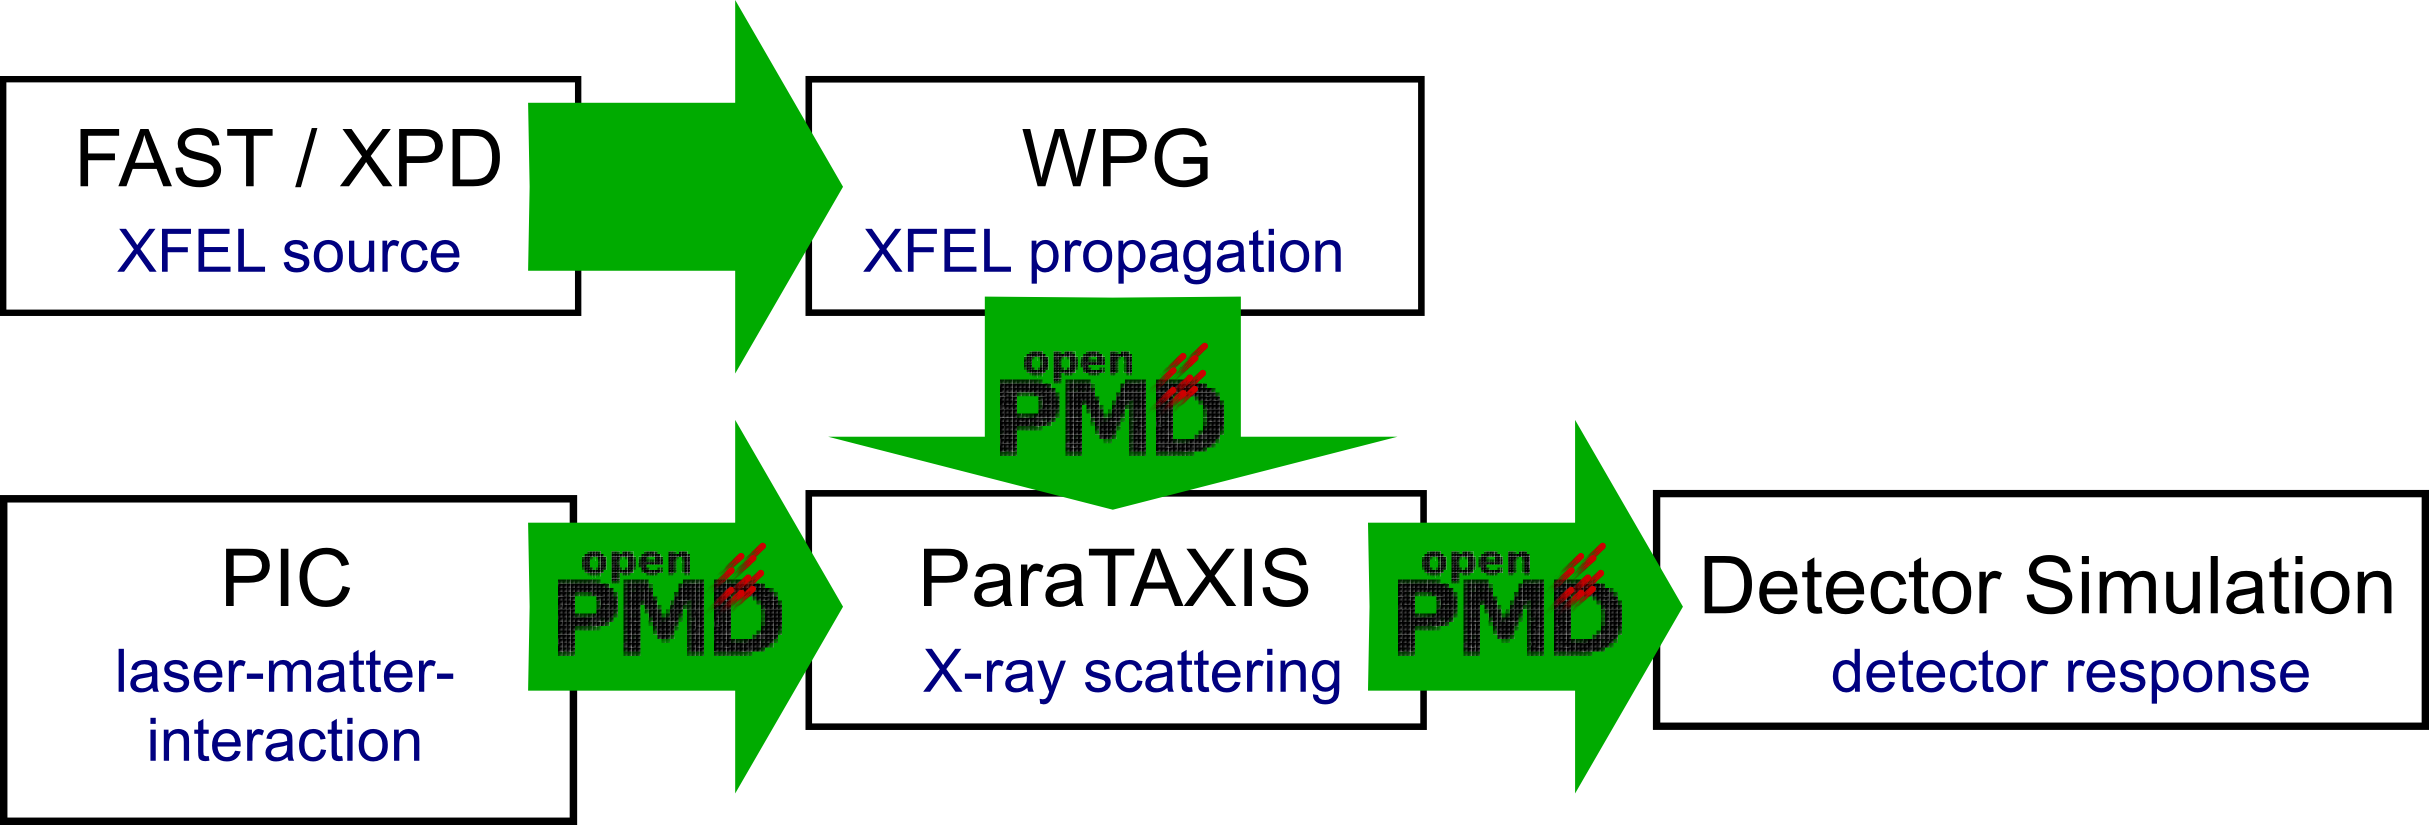
\includegraphics[width=.85\linewidth]{figures/simex_workflow_v2.png}
    \caption{
      SIMEX workflow connecting the simulation codes via data exchange in \textit{openPMD} standard.
    }
    \label{fig:workflows}
  \end{figure}
%
Thus, radiation transport calculations must take these time and length scales
into account. We here introduce the example of softening and expansion of a
grating structure, see Fig. \ref{fig:density},  that is irradiated by an \gls{uhi}
optical laser pulse to illustrate the possibilities of \textit{ParaTAXIS}, a tool
developed within WP4 that resolves radiation transport on the single photon
level. \textit{ParaTAXIS} is fully integrated into the \textit{simex\_platform} tool chain via
\textit{openPMD} \cite{Huebl2017} in- and output, see Fig. \ref{fig:workflows}.

We study a $\tau_\mathrm{opt} = \SI{83}{\fs}$ \gls{fwhm} duration, wavelength $\lambda_\mathrm{opt} =
\SI{0.8}{\micro\metre}$ laser pulse impinging on a silicon foil under oblique incidence
that drives the grating into a heated plasma state. An x--ray pulse of
$\tau_\mathrm{XFEL} = \SI{10}{\fs}$ (\gls{fwhm}) with photon energy
$E_\mathrm{XFEL} = \SI{8.4}{\kilo\electronvolt}$ probes the surface grating structure
perpendicularly to the optical laser propagation with a delay relative to its
pulse maximum arriving at the target surface. With growing delay we expect the
scattering maxima of the grating to vanish as its edges soften and the plasma
expands into the vacuum.
%
\begin{figure}[ht]
  \centering
  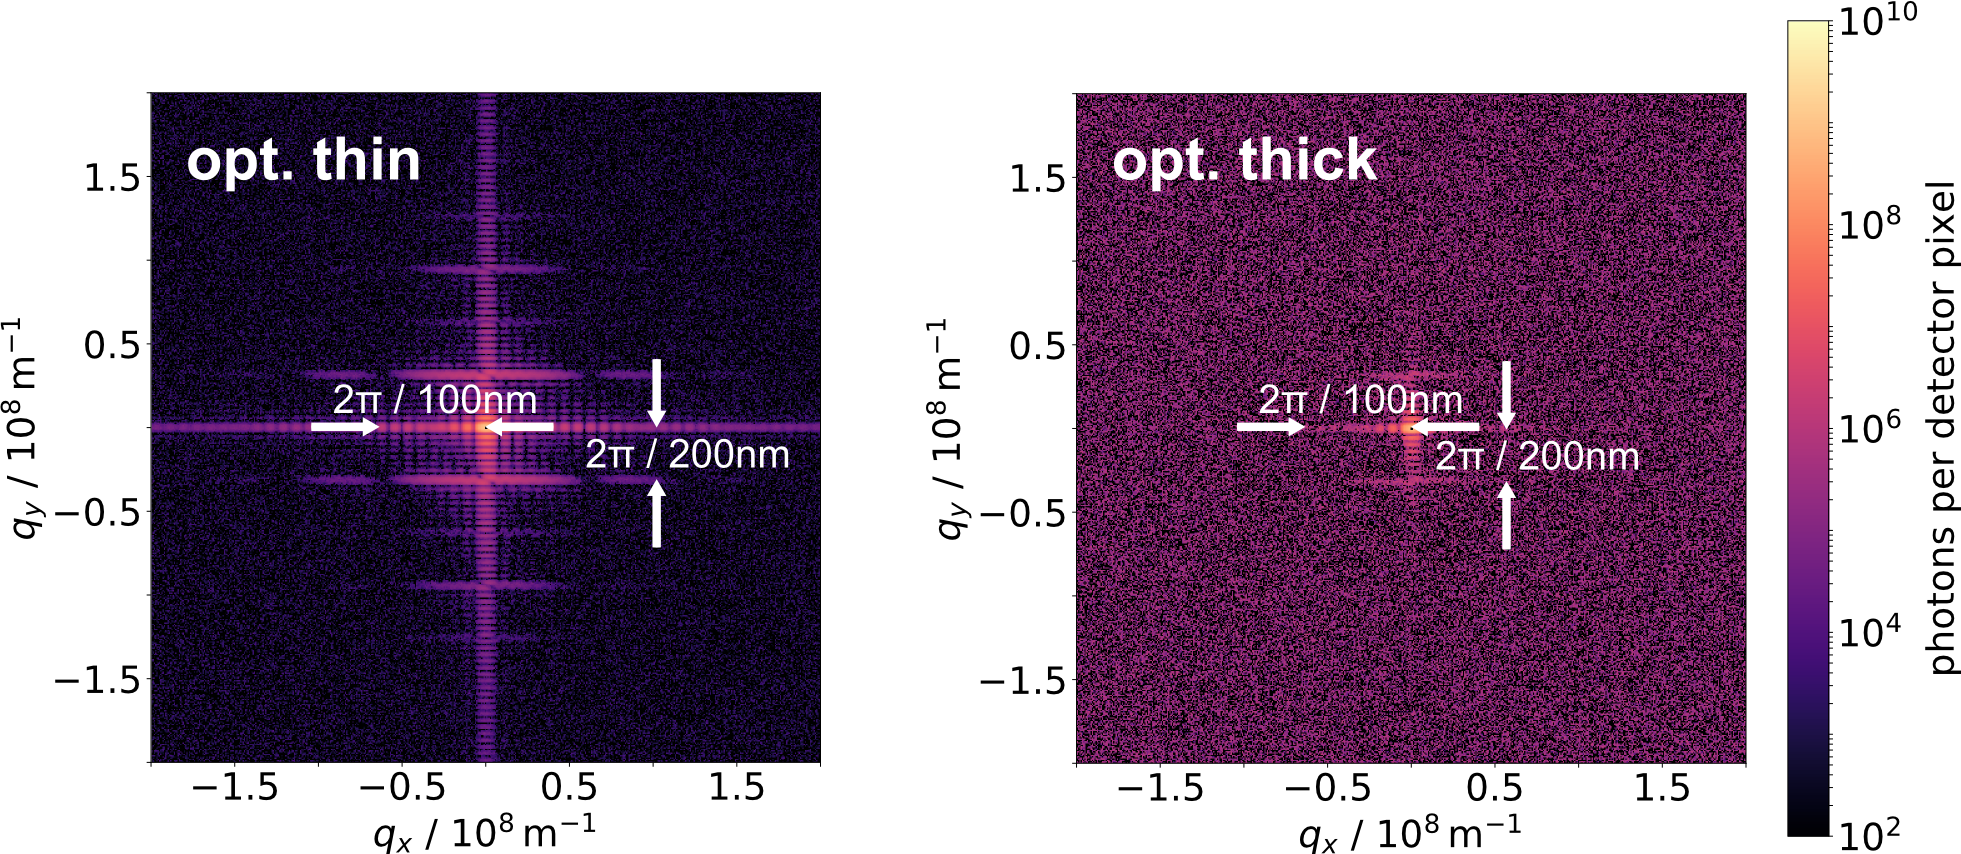
\includegraphics[width=.99\linewidth]{figures/scattering_images_v2.png}
  \caption{
    \textbf{Left:} \textit{ParaTAXIS} \gls{saxs} image for the optically thin target at
    $\SI{1.4}{\metre}$ distance from the target, detector pixel size $a_D =
    \SI{13.5}{\micro\metre}$, X-ray wavelength $\lambda_\mathrm{\gls{xfel}} =
    \SI{1.47}{\angstrom}$ and
    \num{e12} photons in the illuminated area. The vertical separation of scattering
    lines corresponds to the grating period of \SI{200}{\nano\metre}, the horizontal to
    the grating depth of \SI{100}{\nano\metre}.
    \textbf{Right:} \textit{ParaTAXIS} \gls{saxs} image for the optically thick target. Here, the
    scattering cross section was increased by a factor of \num{1000} to account for
  resonant scattering at the ion density. All other parameters remain the same.  }
  \label{fig:scattering}
\end{figure}
%
The time structure of the \gls{xfel} pulse, the evolution of the target while the
pulse probes it and effects like multiple-scattering smear out the scattering
maxima. All effects are taken into account by \textit{ParaTAXIS}.
Details of the signal generation using \textit{ParaTAXIS} for two cases (optically thin and optically
thick target) are presented in the Deliverable Report D4.4
\cite{EUCALL_SIMEX_D4.4}. We show here the resulting scattering images in
Fig.~\ref{fig:scattering}.

\FloatBarrier



\section{\Gls{xafs}\label{sec:xafs}}
%
We have executed the simulations outlined in Deliverable
4.2\cite{EUCALL_SIMEX_D4.2}, describing an XAFS experiment on shock compressed
solid matter. There are three areas of simulation that are considered to describe the
whole source-to-end experiment: X-ray source \& ray tracing, long pulse photon-matter
interaction, and X-ray absorption modelling. Currently, the simulations of X-ray
source/X-ray tracing and XAS modelling are standalone simulations that provide
important information for the long pulse hydrocode simulations. Information
such as X-ray beam size on sample, will influence the laser conditions that can
be accepted for hydrocode simulation (the laser spot must be larger than the
X-ray spot size).

\subsection{Synchrotron x--ray source and ray tracing}
The synchrotron x--ray source and propagation from the source to the target is
realized with the
\href{http://ftp.esrf.eu/pub/scisoft/Oasys/readme.html}{\textit{Oasys}}
software package using the x--ray tracing
code \textit{Shadow3}. Installation scripts and the wiki page for \textit{Oasys} can be
found at
\href{https://github.com/srio/oasys-installation-scripts/wiki}{https://github.com/srio/oasys-installation-scripts/wiki}.
\href{https://github.com/srio/ShadowOui-Tutorial}{Tutorials for
Oasys and ShadowOUI} cover the various steps in preparing, executing, and
analysing the raytracing simulation. As part of preparation for the new High Power
Laser Facility (HPLF), that will be installed on the ID24 beamline at the ESRF,
the current energy dispersive x--ray absorption beamline has been simulated using
\textit{Oasys}.
The ID24 beamline workflow for \textit{Oasys} can be obtained from the EUCALL Data
Repository at Zenodo \cite{Briggs2017.zenodo.886451}.

\subsection{Particle matter interaction: long pulse laser}
The long pulse laser interaction with the sample is performed using the
radiation--hydrodynamics simulation code \textit{Esther} \cite{Colombier2005}.
Here we have demonstrated an experiment that could be performed on the
ID24 \gls{xas} beamline, where a \SI{6}{\nano\second} flat top laser pulse (wavelength
\SI{1064}{\nano\metre}) sends an ablative
driven shockwave through a \SI{45}{\micro\metre} CH-plastic ablator and into a
\SI{5}{\micro\metre} Fe layer. A
tutorial that describes how the input files are generated (and how output data is
obtained) is provided on the
\href{https://www.github.com/eucall-software/simex_platform/wiki/Esther-Hydrocode-Tutorial}{\textit{simex\_platform} wiki page}; all example input
and output files are available from the Ref.~\cite{Briggs2017.zenodo.883106}.
The pressure in the Fe sample at $t = \SI{8.9}{\nano\second}$
(laser pulse begins at $t = \SI{0}{ns}$) is shown in Fig.~\ref{fig:hydro}.

 The pressure, temperature, density and velocity can all be obtained at any given
 time step from the output files that Simex converts to OpenPMD \cite{Huebl2017} format. Upon
 completion of the code, it is then possible to adjust the laser parameters to reach
 different pressure-temperature conditions in the Fe sample. The P-T condition
 where the pressure is uniform through the whole of the sample is then recorded and
 \gls{xas} modelling can be performed to simulate the expected E\gls{xafs} signal at
 the compressed state.
%
 \begin{figure}
   \centering{%
     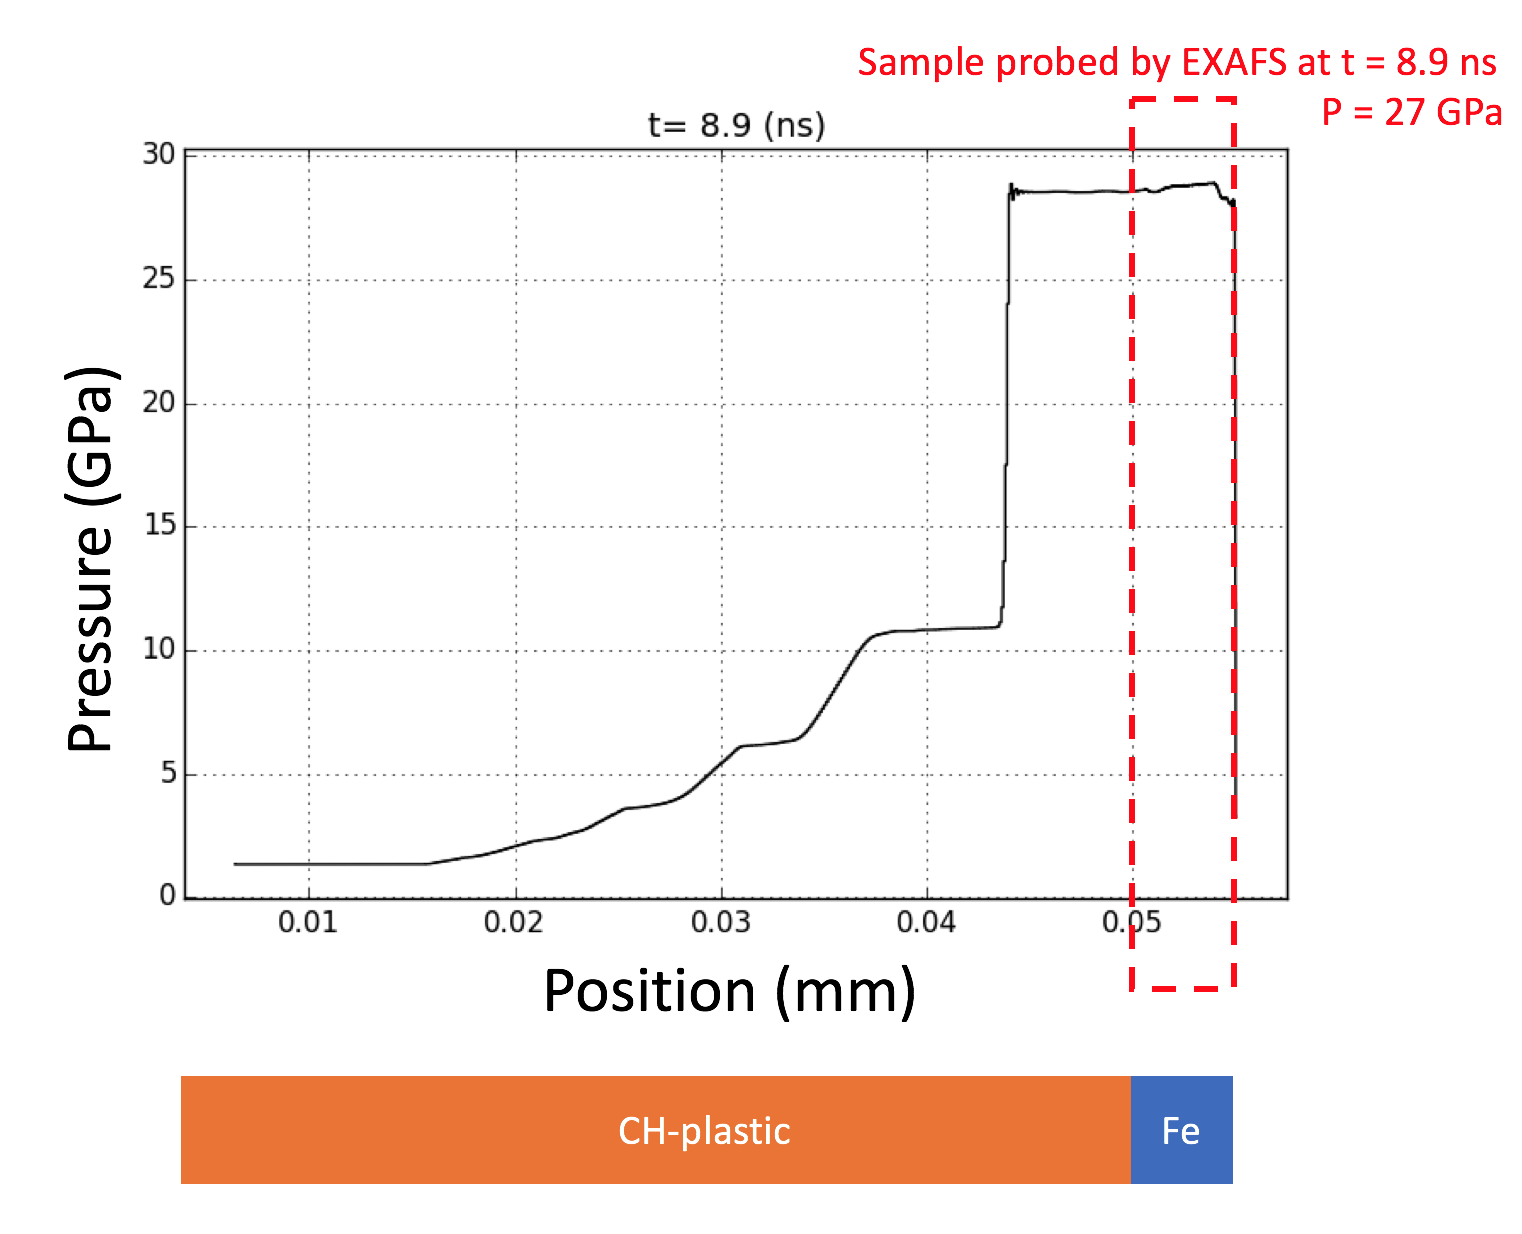
\includegraphics[width=4.822in]{figures/SIMEX-Fe-Shock.png}
     \caption{%
       Pressure distribution in the plastic ablator layer (0-0.05 mm) and iron sample
(0.05-0.055 mm). The laser arrives at 0 mm and sends the shock wave through the plastic. Upon reaching the
Fe layer the shock pressure jumps to ~ 30 GPa and sends a reshock wave back into the plastic. The red-dashed
box highlights the iron sample that is probed by the X-rays.  \label{fig:hydro}}
   }
 \end{figure}
%
 \subsection{Modelling of \gls{exafs}}
In this example, to show the interoperability with the hydrocode,
we run through the requirements that are necessary for
simulation (fitting) of \gls{exafs} data relevant to obtain signal
from a \SI{5}{\micro\metre} thick Fe foil. The simulation will be carried out for
ambient conditions Fe foil; a future enhancement of SIMEX will take P-T
conditions from hydrocode simulations before performing high-pressure
\gls{xanes}/\gls{exafs} calculations.

To validate the \gls{exafs} simulations, we compare the simulated spectrum with raw
data obtained from an \gls{xas} beamline at the ESRF synchrotron. The
normalized \gls{xas} spectrum for a \SI{5}{\micro\metre} thick Fe foil is shown in
Fig.~\ref{fig:hydro}.
%
\begin{figure}
  \centering{%
    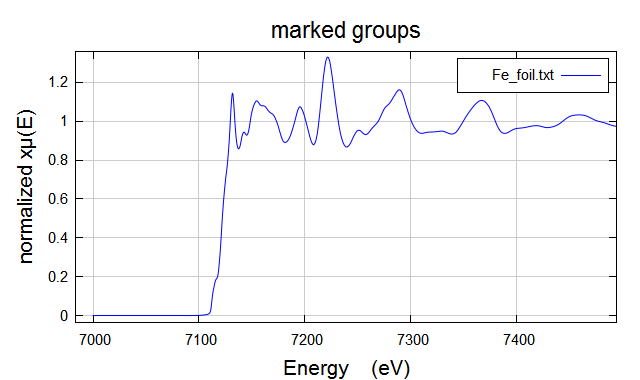
\includegraphics[width=4.822in,height=2.528in]{figures/Task42210-img001.png}
    \caption{%
      X--ray absorption spectra collected at BM23 (\gls{exafs} beamline, ESRF) of
      a \SI{5}{\micro\metre} thick iron foil.
      \label{fig:xafs_spectra}
    }
  }
\end{figure}
%
Calculations of \gls{xafs} spectra are performed using the \textit{FEFF} package
\cite{Rehr2009}. \textit{FEFF} uses a
single input file to select which modules should be run inside the program and
what parameters should be used. The material of interest is contained within
this input file based on its crystallographic parameters and atomic positions.
The \textit{ATHENA} program is able to combine crystallographic input files (.cif format)
for a chosen material into the \textit{FEFF} .inp format. The .cif files can be
found on crystallographic database websites or can be manually created
using gui programs such as \textit{VESTA}. \textit{FEFF} is then run to
calculate the scattering paths
between atoms and the run data is then exported for use by other third party programs
(such as \textit{ARTEMIS}) to compare with experimental data.
A comprehensive user guide for running ARTEMIS
/ \textit{FEFF} can be found at\\
\href{http://bruceravel.github.io/demeter/artug/index.html}{http://bruceravel.github.io/demeter/artug/index.html}.
%
\begin{figure}
  \centering{%
    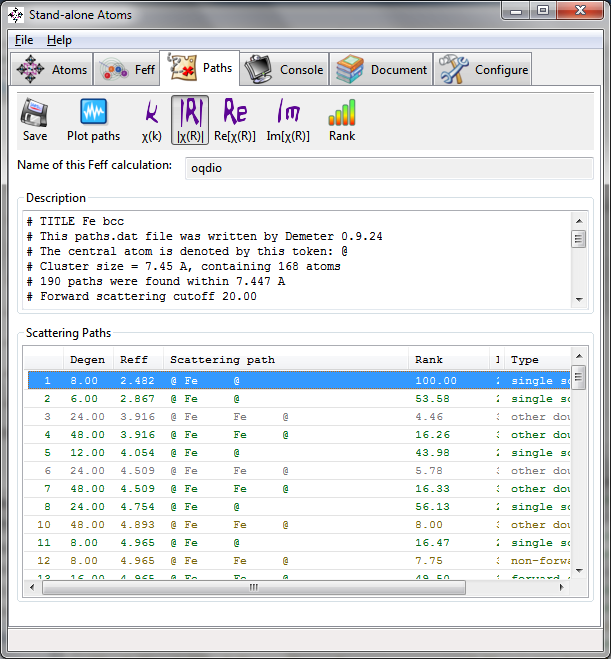
\includegraphics[width=4.3063in,height=4.6465in]{figures/Task42210-img002.png}
    \caption{%
      Screenshot of the output data collected in the ATOMS software after
      running \textit{FEFF} simulation of iron at ambient conditions.
      \label{fig:xafs_fig2}
    }
  }
\end{figure}
%
\begin{figure}
  \centering{%
    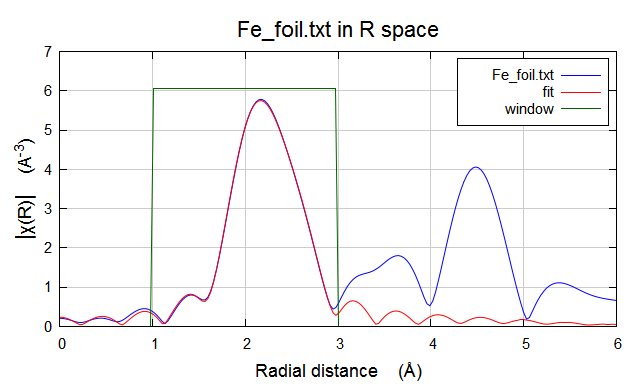
\includegraphics[width=4.852in,height=2.9173in]{figures/Task42210-img003.png}
    \caption{%
      Fitting of the first Fe shell from \textit{FEFF} calculations (red) to Fe
      \gls{exafs}
      data collected on BM23 beamline, ESRF (blue).
      \label{fig:xafs_fig3}
    }
  }
\end{figure}
%
\subsubsection{Simulating \gls{xanes} at shock conditions}
Shock compression experiments on Fe have previously been carried out at the ESRF
\cite{Torchio2016}. In that study,
simulations of the \gls{xanes} at shock conditions were carried out using the
\textit{abinit} code and are shown below in Fig.~\ref{fig:xafs_fig4}.
%
\begin{figure}
  \centering{%
    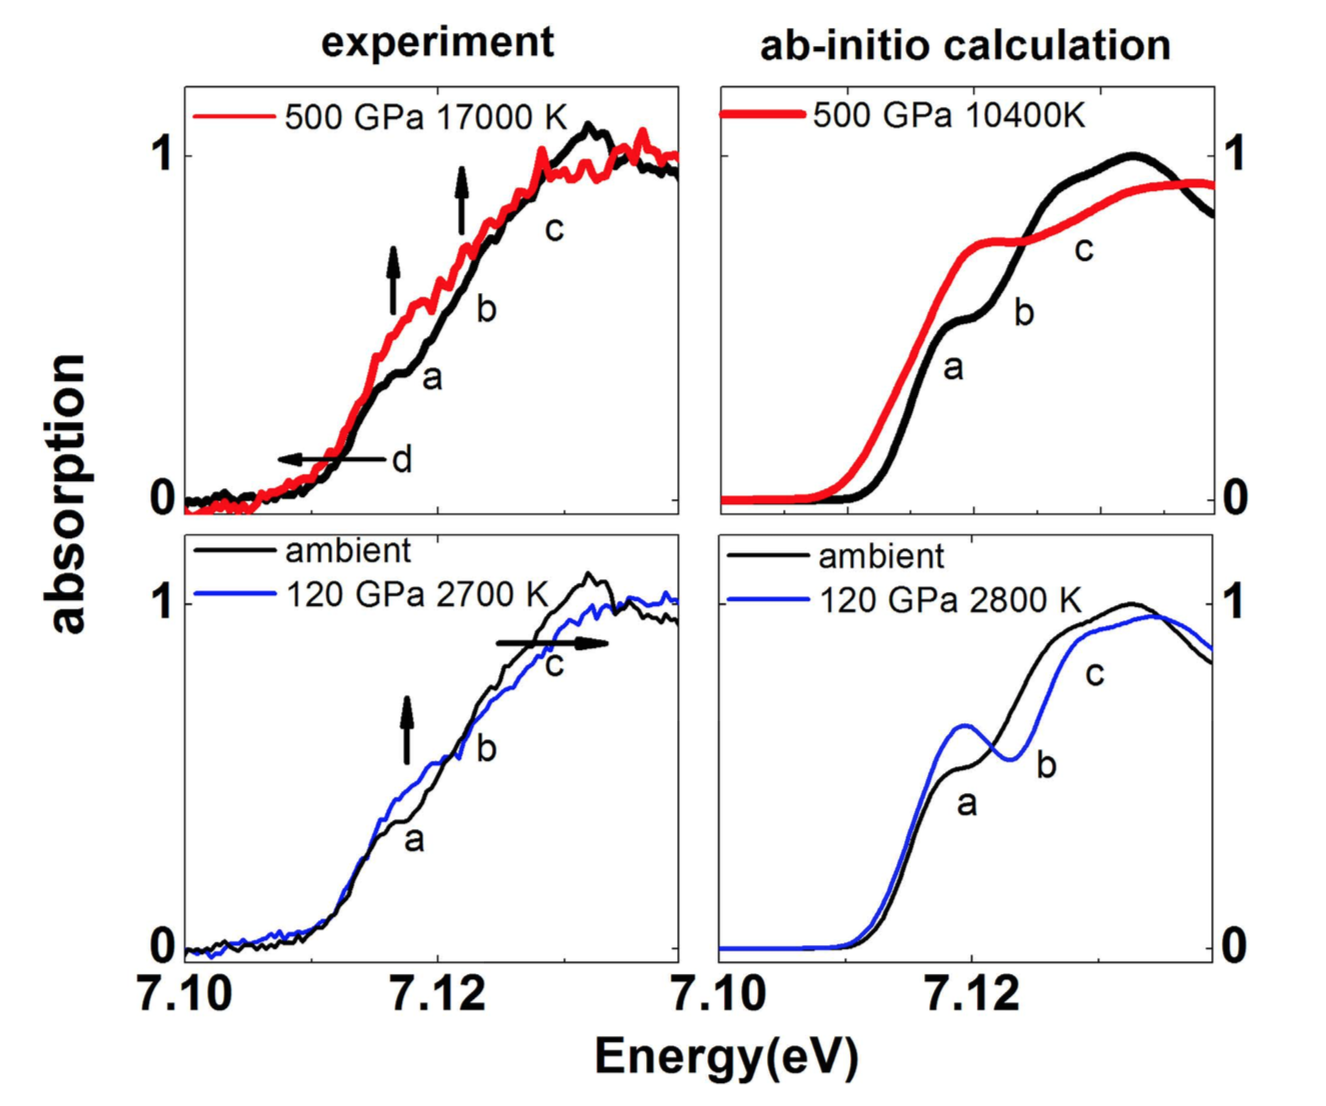
\includegraphics[width=4.3063in,height=3.5945in]{figures/Task42210-img004.png}
    \caption{%
      Comparisons of the absorption edge of Fe between experiments (left
      panels) and ab-initio calculations (right panels) at
      \SIlist{120;150}{\giga\pascal}. Figure
      taken from Ref.~\cite{Torchio2016}.
      \label{fig:xafs_fig4}
    }
  }
\end{figure}


\href{https://www.github.com/eucall-software/simex_platform/wiki/Esther-Hydrocode-Tutorial}{A
documented example workflow} is provided to demonstrate the usability of the
radiation--hydrodynamics simulation capabilities in \textit{simex\_platform}. It
shows how to optimize the target geometry (i.e. the thickness of the ablator
material) to maximize the data output, making use of the openPMD metadata
standard to facilitate transferability among involved simulation codes and
data analysis and visualisation tools.
%
\section{Coherent diffraction from protein nano--crystals\label{sec:protein_sfx}}
In an
\href{https://github.com/eucall-software/simex_platform/wiki/Tutorial-on-nano-crystal-diffraction}{online
tutorial}, we demonstrate the usage of \textit{simex\_platform} to simulate
coherent diffraction of XFEL photons from nano--metre scale crystalline samples.
As in the other XFEL applications (see Sec.~\ref{sec:plasma_diffraction} and
Sec.~\ref{sec:xrts} as well as the first demonstration example in Milestone
M4.2 \cite{EUCALL_SIMEX_M4.2}), the source wavefront is queried from the
\href{https://in.xfel.eu/xpd}{XFEL Pulses Database XPD} and propagated to the
sample interaction point in the focus of the SPB--SFX instrument by means of
the coherent wavefront propagation code library WPG. Owing to the well defined
data interfaces and file format adaptors in \textit{simex\_platform} passing the
wavefront data to the crystal diffraction code is straightforward. We employ the
code \textit{pattern\_sim} which is part of the crystallography software suite
\textit{CrystFEL} \cite{White2012}, available as open source from the
\href{https://www.desy.de/~twhite/crystfel}{CrystFEL website}. The
corresponding \textit{Calculator} in \textit{simex\_platform} is the
\href{https://eucall-software.github.io/simex_platform/#SimEx.Calculators.CrystFELPhotonDiffractor.CrystFELPhotonDiffractor}{\textit{CrystFELPhotonDiffractor}}.
The \textit{CrystFELPhotonDiffractor} extracts the mean photon energy, the energy
spectrum, the beam divergence, the beam diameter, and other beam characteristics
from the wavefront data. The sample must be specified by giving a PDB code along
with information about the size of the nano--crystal, e.g. the extension in x,y,
and z directions. By default, the sample geometry is rotated in space via a
randomly chosen rotation operator to mimic the unknown orientation of the sample
in the experiment. Each simulated pattern is stored in a separate hdf5 file.
After the calculation, one master hdf5 file is generated which links to the
individual patterns and which has the same hierarchy as output generated e.g. by
the
\href{https://eucall-software.github.io/simex_platform/#SimEx.Calculators.SingFELPhotonDiffractor.SingFELPhotonDiffractor}{\textit{SingFELPhotonDiffractor}}
for single particle coherent diffraction. This in turn ensures that the same
analysis tools (e.g.
\href{https://eucall-software.github.io/simex_platform/#SimEx.Analysis.DiffractionAnalysis.DiffractionAnalysis}{\textit{DiffractionAnalysis}})
can be applied to crystal diffraction data and to single particle diffraction
data.
%
\section{Plasma X--ray Thomson Scattering\label{sec:xrts}}
%
X--Ray Thomson Scattering (XRTS)~\cite{Glenzer2009,Fortmann2009d} has
become an important method for the diagnosis of matter at extreme conditions of
temperature and density. These quantities can be inferred from the spectrally
resolved scattering intensity if the spectrum was measured with high resolution.
The resolution primarily depends on the detector's point spread function, the
energy resolution of the dispersive element, and on the spectral width of
the probe radiation. Complex structured source spectra, e.g. K--shell multiplets
\cite{Lee2009a} or saturated SASE (self--amplified spontaneous emission) spectra
limit the accuracy to which plasma properties can be measured.

XRTS can now be simulated within \textit{simex\_platform}. The corresponding
\textit{Calculator} is the
\href{https://eucall-software.github.io/simex_platform/#SimEx.Calculators.PlasmaXRTSCalculator.PlasmaXRTSCalculator}{\textit{PlasmaXRTSCalculator}},
the backengine simulation code is called \textit{xrs} and can be obtained by
request from the maintainers of \textit{simex\_platform}. The
\href{https://eucall-software.github.io/simex_platform/#SimEx.Calculators.PlasmaXRTSCalculator.PlasmaXRTSCalculator}{\textit{PlasmaXRTSCalculator}}
accepts wavefront data from the
\href{https://eucall-software.github.io/simex_platform/#SimEx.Calculators.XFELPhotonPropagator.XFELPhotonPropagator}{\textit{XFELPhotonPropagator}}
from which it will extract the power spectrum of the scattering photons and
convolute it with the dynamic structure factor coming from the \textit{xrs}
code.

A tutorial and example demonstration has been added to the
\href{https://github.com/eucall-software/simex_platform/wiki/XRTS-Tutoria}{simex\_platform
wiki}. It explains how to setup the source, propagation and XRTS calculation
to generate scattering spectra with explicit account for the source spectrum.

Fig.~\ref{fig:xrts_spectrum_and_source} demonstrates the impact of a broad SASE
spectrum on the simulated \gls{xrts} spectrum. Here, we used a propagated
wavefront from the SASE1 beamline at European XFEL of \SI{3}{\femto\second}
duration and \SI{5}{\kilo\electronvolt} photon energy. The simulation of the FEL
source was performed at high saturation leading to the numerous SASE spikes and
rather broad spectral width of the x--ray probe.

\begin{figure}[ht]
  \begin{center}
    \subfloat[]{%
    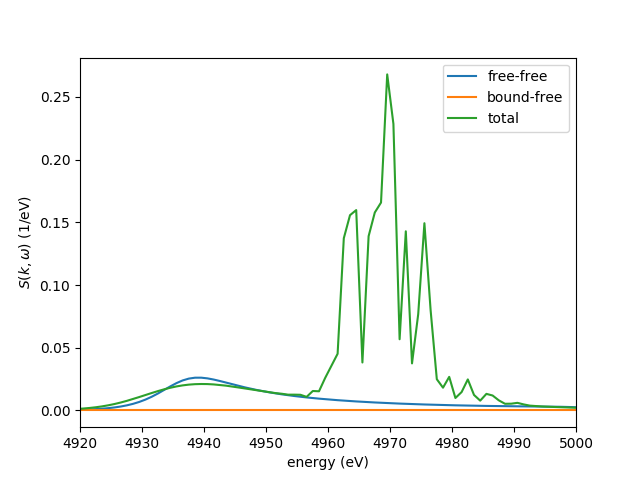
\includegraphics[width=0.8\textwidth,angle=0,clip]{figures/Be_30deg_5keV_RPA.png}
    \label{fig:xrts_spectrum}
  }\\
  \subfloat[SASE spectrum]{%
    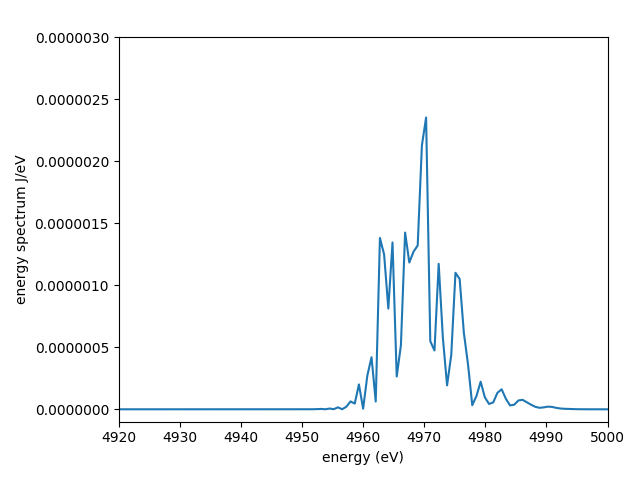
\includegraphics[width=0.8\textwidth,angle=0,clip]{figures/SASE1_5keV_3fs_spectrum.png}
    \label{fig:xrts_source}
  }
  \end{center}
  \caption{(a) \gls{xrts} spectrum showing free--free, bound--free, and elastic
  scattering. The source spectrum (b) determines the spectral shape of the elastic
feature and smears our the inelastic features.}
  \label{fig:xrts_spectrum_and_source}
\end{figure}

In Ref.~\cite{Rozmus2017_submitted}, the theoretical models to describe
scattering from weakly collisional plasmas implemented in \textit{xrs} are
benchmarked against a plasma kinetic model. A second publication, analysing the
range of applicability of the so--called impulse approximation for Compton
scattering from bound states is currently in preparation \cite{Bell2017_prep}.
%
\FloatBarrier

%
\section{Laser--plasma accelerator driven FEL source}\label{sec:lwfa_source}
%
Simulations of compact coherent x--ray sources based on the mechanism of
electron laser wakefield acceleration  couple particle--in--cell
simulations to an \gls{fel} code. In our case, we use the \gls{pic} code \textit{PIConGPU}
and the \textit{Genesis} \gls{fel} code, both are publicly available under open source licenses.
\textit{PIConGPU} writes the particle and field data
into a hdf5 file using the openPMD \cite{Huebl2017} metadata standard. A file format conversion utility, which is part of
\textit{simex\_platform} converts the \gls{pic} output to an electron distribution
file (extension .dist) readable by \textit{Genesis}.


This interface was used to investigate the possible
route for the experimental realization of a laser plasma accelerator based coherent
light source \cite{Emma2004}. \Glspl{lpa}~\cite{Leemans2006,Esarey2009,Tajima1979} have the potential to become the next
generation of accelerator facilities reaching field gradients of the order of
\SI{100}{\giga\electronvolt\per\metre}, i.e. up to three orders of magnitude
higher than in conventional linear accelerators. This would reduce construction
and operation costs by comparable orders of magnitude.

\subsection{Start--to--end simulation of \gls{lpa} based \glspl{fel}\label{sec:lwfa_s2e}}
Our simulation setup is shown in Fig.~\ref{fig:lwfa-setup}; starting from electron
beam generation from a laser plasma source to the generation of femtosecond
and/or attosecond EUV/XUV pulse from the radiation undulator.
%
\begin{figure}[ht]
  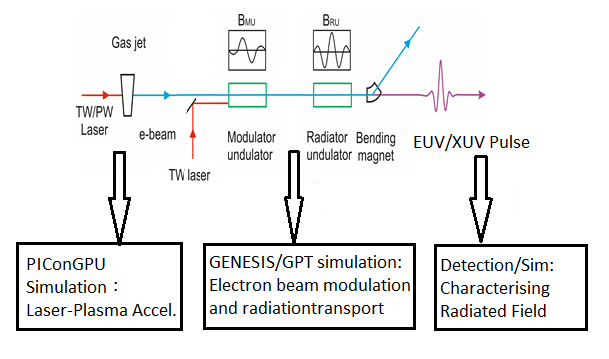
\includegraphics[width=5.4165in,height=2.7374in]{figures/lwfafel-img001.png}
  \caption{Scheme of \gls{lpa}--\gls{fel} simulation}
  \label{fig:lwfa-setup}
\end{figure}
%
In this scheme an intense
\SIrange{10}{100}{\tera\watt}
laser is focused onto a gas jet or a gas filled capillary for producing a
relativistic electron beam. Initial energy spread of the electron beam of a
\gls{lpa} (\numrange{1}{5}\%) is typically much larger than that of a linear accelerator
(about \num{0.05}\%), so
reduction of the slice energy spread is necessary. The electron beam is sent
through a modulator undulator (MU) together with a TW--power laser beam, where
the interaction between the electrons, the magnetic field of the undulator and
the electromagnetic field of the laser introduces a periodic energy modulation
of the electrons. This energy modulation leads to the formation of nano--bunches
(ultrashort electron layers). The nano--bunched electron beam then passes through
a radiator undulator (RU) consisting of a single or a few periods and creates
EUV/XUV pulses.
%
The SIMEX setup (as shown in Fig.~\ref{fig:lwfa-setup}) for a \gls{lpa} driven \gls{fel}
utilizes the \textit{PIConGPU} simulation code for electron beam generation using the \gls{lpa}
mechanism and further transportation of electron beam to the \gls{fel} simulation.
We show a schema of the iterative SIMEX workflow in
Fig.~\ref{fig:lwfa-simulation_loop}. We start by defining the initial laser--plasma
parameters and initial conditions for \textit{PIConGPU}.
\textit{PIConGPU} computes the 6D electron beam distributions at the rear
side of the plasma in vacuum. The obtained electron beam distribution is
transformed via a python script to a distribution file (.dist) for
\textit{GENESIS}). \textit{GENESIS} calculates the electron beam dynamics
induced by the magnetic field distribution. The output data file from
\textit{GENESIS} can be further post--processed to calculate and visualize the radiation
field.

An online tutorial, demonstrating how to use the simulation capabilities and
data format converters will be added to the \textit{simex\_platform} wiki pages
soon. Generation of production simulation data for a realistic case study
is currently hindered by the unavailability of sufficient computing resources.
In order to simulate SIMEX for LPA driven FEL; we need adequate computing resources to run PIConGPU simulations for generation of high quality electron beam; a necessary condition for FEL radiation. At the moment, available GPUs for computation are short in numbers; subsequently we are unable to present the data in this report. A
proposal for compute time at a high performance computing facility (e.g. within the
PRACE) network) is currently being prepared.
\begin{figure}[ht]
  \begin{center}%
    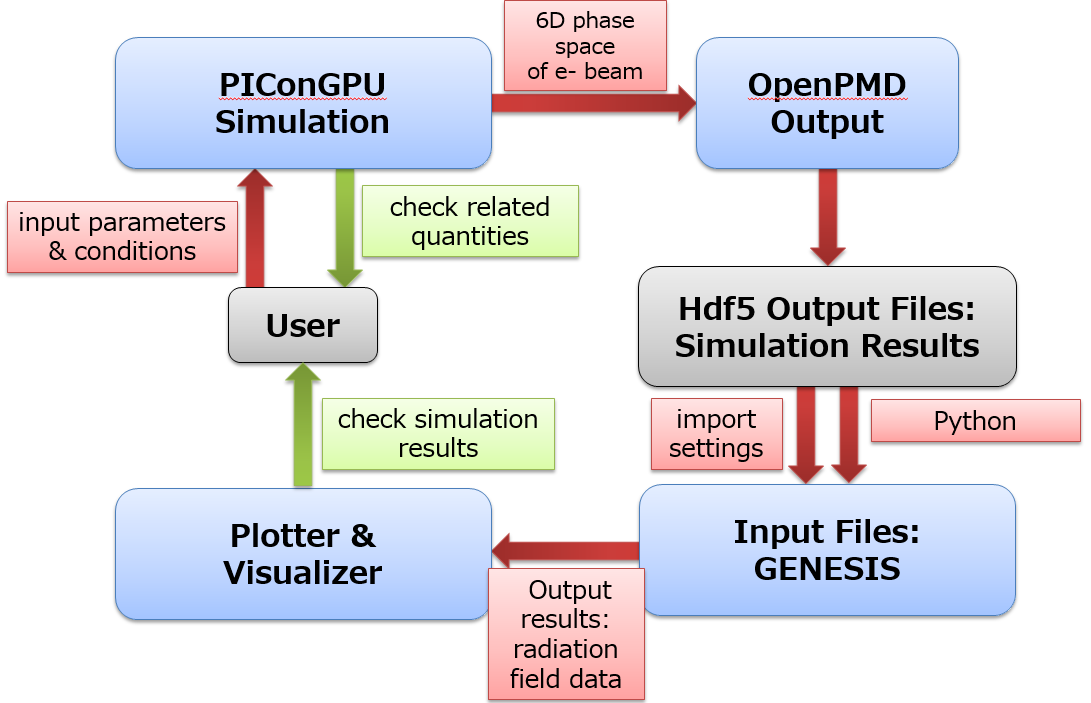
\includegraphics[width=5.9425in,height=4.1882in]{figures/lwfafel-img002.png}
    \caption{Layout for simulation setup and feedback loop}
    \label{fig:lwfa-simulation_loop}
  \end{center}%
\end{figure}
%
\subsection{Laser--plasma accelerator based single--cycle attosecond undulator source}
In parallel, we have studied\footnote{This study was performed in collaboration
with T. Zoltan and Prof. Hebling, both at Pecs University, Hungary.} the feasability of a \gls{lpa} based coherent light
source using experimental data for electron wakefield acceleration as input to
the \gls{fel} simulation. The \gls{fel} simulation used the code \textit{GPT} in this case.
Details are discussed in Ref.~\cite{Tibai2017}.

Fig.~\ref{fig:Tibai2017} displays the simulated waveform (electric field as
a function of time)  of the generated attosecond
pulse and the beam profile at \SI{60}{\nano\metre} radiation wavelength. The
temporal evolution was measured on the axis of highest intensity, marked by  a
cross in Fig.~\ref{fig:Tibai2017_profile}. At other wavelengths, the shape of the attosecond pulses are nearly identical with the
shape shown in Fig.~\ref{fig:Tibai2017_E_vs_t}, showing that these pulses are
\gls{cep} controlled \cite{Tibai2017}.
%
\begin{figure}[ht]
  \centering{%
    \subfloat[]{
      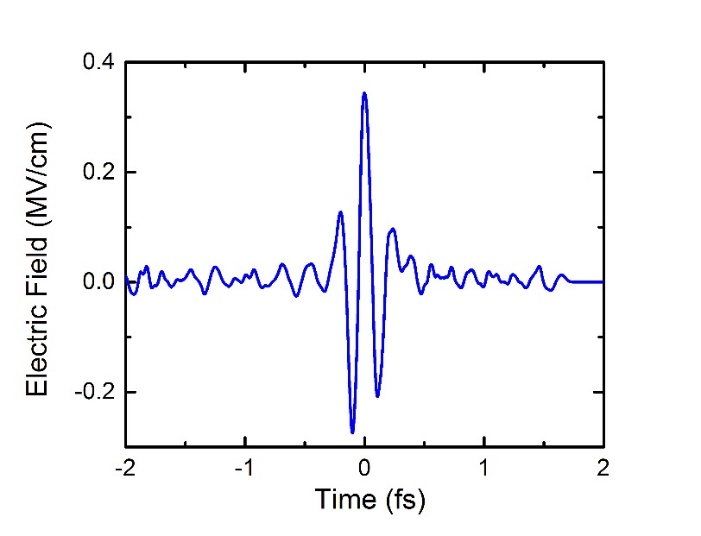
\includegraphics[width=2.7016in,height=2.1583in]{figures/lwfafel-img003.jpg}
      \label{fig:Tibai2017_E_vs_t}
    }
    \subfloat[]{
      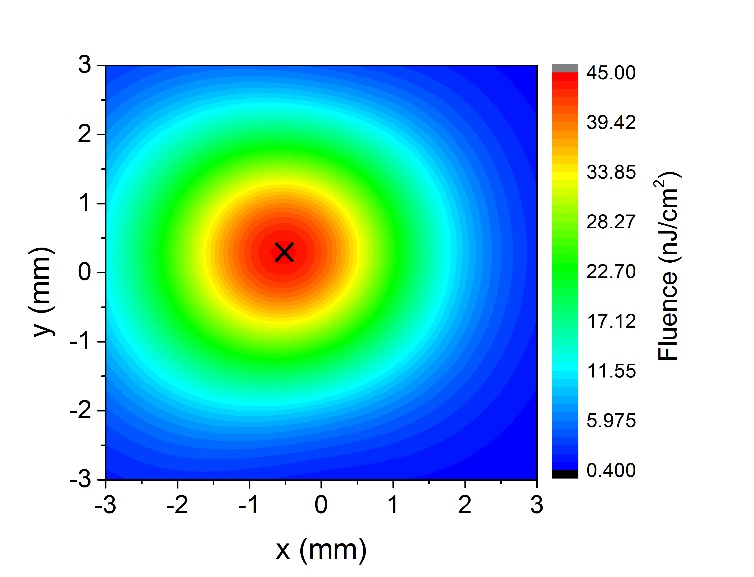
\includegraphics[width=3.0083in,height=2.352in]{figures/lwfafel-img004.jpg}
      \label{fig:Tibai2017_profile}
    }
  }
  \caption{GPT Simulation Results: \gls{cep}--controlled \gls{euv} waveforms (left) and its spatial beam
    profile (right).}
    \label{fig:Tibai2017}
\end{figure}



%%%%%%%%%%%%%%%%%%%%%%%%%%%%%%%%%%%%%%%%%%
% No floating objects beyond this point. %
%%%%%%%%%%%%%%%%%%%%%%%%%%%%%%%%%%%%%%%%%%
\FloatBarrier

\section{References}
%
\printbibliography[notkeyword=submitted, notkeyword=inpreparation, notkeyword=report, notkeyword=zenodo, title={Journal articles}]
%
\printbibliography[keyword=submitted, title={Submitted articles}]
%
\printbibliography[keyword=inpreparation, title={Articles in preparation}]
%
\printbibliography[keyword=eucall, keyword=report, title={EUCALL reports}]
%
\printbibliography[keyword=zenodo, title={Zenodo depositions}]

\end{document}

